\section{A Programação Linear e as suas Aplicações}
Na pesquisa operacional, a programação linear é uma das técnicas mais utilizadas em problemas de otimização. Os problemas de programação linear geralmente buscam a distribuição eficiente de recursos limitados para atender um determinado objetivo, por isso suas aplicações estão presentes em diversas áreas como computação, administração, indústria e transporte \cite{Engecom}.

Um problema de programação linear é expresso através de um modelo que é composto por equações e inequações lineares. Esse tipo de problema busca a distribuição eficiente de recursos com restrições para alcançar um objetivo, em geral, maximizar lucros ou minimizar custos. Em um problema de programação linear esse objetivo é expresso através de uma equação linear denominada função objetivo. Para a formulação do problema, é necessário também definir os recursos necessários e em que proporção são requeridos. Essas informações são expressas em equações ou inequações lineares, uma para cada recurso. Esse conjunto de equações ou inequações é denominado restrições do modelo \cite{Engecom}.

\section{Descrição do Problema de Programação Linear}
O modelo de um problema de programação linear normalmente é apresentado em uma das formas a seguir \cite{Passos}:
$\\Max\ z = c^{T}x \\\\s.a.\left\{\begin{matrix}
Ax\leq b\\x\geq 0 
\end{matrix}\right.$  

ou  

$\\Min\ z = c^{T}x \\\\s.a.\left\{\begin{matrix}
Ax\geq  b\\x\geq 0 
\end{matrix}\right.$


Um problema de programação linear com até três variáveis pode ser representado graficamente utilizando três eixos cartesianos. Os problemas com duas variáveis podem ainda ser facilmente resolvidos por meio da representação gráfica \cite{Passos}. 

A seguir é apresentado um problema com duas variáveis e sua representação. Apesar de, na prática os problemas de programação linear possuirem um número de variáveis muito maior que dois ou três, a visualização gráfica de modelo, mesmo que simples, contribui para o entendimento dos métodos de resolução apresentados nas seções a seguir.
No problema exemplo, uma empresa, que fabrica vários produtos, deseja maximizar o lucro na venda de 2 desses produtos \cite{Hillier}.

$\\
Maximize\ z=3x_{1}+5x_{2}\\
Sujeito\ a \\
        1x_{1}\leq 4 \; \; \; \; \; \; \; \; \; \; \; \;(a)\\
        2x_{2}\leq \; \; \; \; \; \; \; \; \; \; \; \; \; \; \;(b)\\
        3x_{1}+2x_{2}\leq 8 \; \; \; \; (c)\\
        x_{1}\geq 0, x_{2}\geq 0 $

Onde, 
\begin{itemize}
\item \textbf {$x_{1}$} representa a quantidade do produto 1 produzido em uma semana
\item \textbf {$x_{2}$} representa a quantidade do produto 2 produzido em uma semana
\item \textbf {$z$} representa o lucro total por semana de produção desses dois produtos (em milhões de dólares), sendo o lucro do produto 1 de 3 milhões e o do produto 2 de 5 milhões.
\end{itemize}

E as restrições representam as restrições de tempo de cada máquina utilizada no processo de produção,
\begin{itemize}
\item A equação \textbf {(a)} garante que, durante o processo de produção, cada produto 1 necessita de 1 hora na máquina 1, e a máquina só tem disponível 4 horas por semana
\item A equação \textbf {(b)} garante que, durante o processo de produção, cada produto 2 necessita de 2 horas na máquina 2, e a máquina só tem disponível 12 horas por semana
\item A equação \textbf {(c)} garante que, durante o processo de produção, cada produto 1 necessita de 3 horas na máquina 3, e cada produto 2 necessita de 2 horas na máquina 3, e a máquina só tem disponível 8 horas por semana
\end{itemize}

Graficamente representado o problema ficaria da seguinte forma:
\begin{center}
	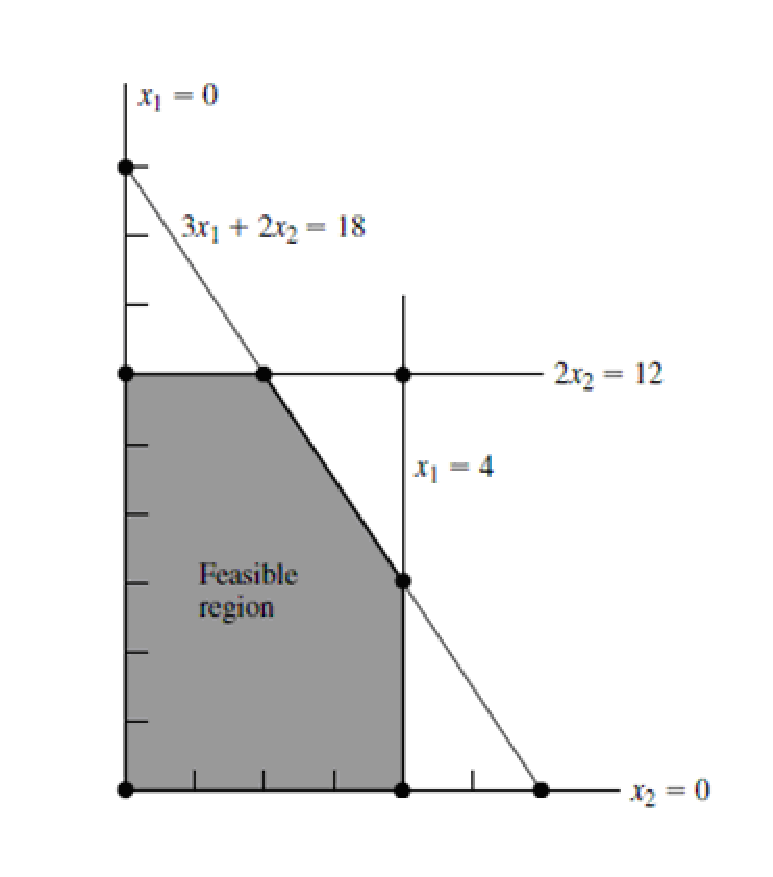
\includegraphics[scale=0.5]{graficos/simplex_grafico}
	\captionof{figure}{Representação gráfica de um Problema de Programação Linear de duas variáveis}
	\label{img:simplex_grafico}
\end{center}

Onde cada reta representa uma restrição do modelo, e a área cinza representa a região viável, ou seja, nessa área estão contidas os valores viáveis de $x_{1}$ e $x_{2}$ para a maximização do lucro.

Os métodos para resolução de problemas de programação linear buscam esses valores de $x_{1}$ e $x_{2}$  para a determinação da solução ótima.

\section{Métodos de Solução}
Entre os métodos mais famosos para a resolução de problemas de programação linear estão o método simplex  e o método de pontos interiores. 
Depois da apresentação do método simplex,outros métodos com diferentes abordagens foram propostos \cite{Todd}. Porém, dentre os métodos existentes apenas o método de pontos interiores é atualmente competitivo em relação ao método simplex \apud{Bixby}{Munari}. 
A principal diferença entre esses dois métodos é o que o método simplex caminha pelos vértices da região viável, enquanto o método de pontos interiores caminha pelo interior da região viável \cite{MaculanPI}. Além disso, uma outra diferença é que o simplex exige muitas iterações com cálculos simples, enquanto no método de pontos interiores poucas iterações são exigidas, porém com cálculos mais elaborados.
Apesar das vantagens do método de pontos interiores em relação ao método estudado neste trabalho, o método simplex possui melhor desempenho na resolução de problemas de pequeno porte em relação ao método de pontos interiores, tornando-se um método indispensável em ferramentas de programação linear.

\subsection{Método Simplex}
O método simplex é um dos algoritmos mais populares para a resolução de problemas de programação linear. Surgiu a mais de 60 anos atrás e foi proposto por George Dantzig.  

É um método iterativo, e sua ideia principal consiste no fato de que a cada iteração uma nova solução é encontrada, sempre melhor que a anterior até o ponto em que a solução ótima é obtida. Outra característica do método é o fato de ser matricial, ou seja, os dados a serem calculados são armazenados em matrizes.  

Com a utilização do método, foi percebido que a cada iteração eram requeridos muitos cálculos sobre valores que nem sempre importavam para a iteração seguinte, fato que do ponto de vista computacional tornaria o método ineficiente. Esse método é chamado de método simplex padrão ou tabular. A partir desse fato foi desenvolvido o método simplex revisado visando a resolução de problemas de programação linear computacionalmente.

%\section{Origem do Método Simplex}
O método simplex surgiu nos Estados Unidos e foi proposto pelo matemático George Dantzig. Quando trabalhava no Pentágono recebeu dos seus colegas o desafio de tentar mecanizar o processo de planejamento. No ano de 1947 Dantzig propôs o método simplex que tornou possível a solução de problemas de otimização de vários tipos, como transporte, produção, alocação de recursos e problemas de escalonamento \cite{OrigemSimplex}.

%\section{Descrição do Método}
\section{Princípio Básico do Método}
A idéia do método simplex consiste em resolver repetidas vezes um sistema de equações lineares, e assim obter uma sucessão de soluções até encontrar a solução ótima. Ou seja, é um processo onde nos movemos de uma solução viável para outra sempre melhor ou pelo menos não pior.

Um problema de programação linear é sempre constituído de uma função objetivo e várias restrições. Geometricamente, essas restrições resultam em uma forma geométrica, chamada hiperplano, no espaço n-dimensional sendo n o número de variáveis no modelo. E cada vértice desse hiperplano é considerado uma solução viável, como ilustra o exemplo abaixo.
\begin{center}
	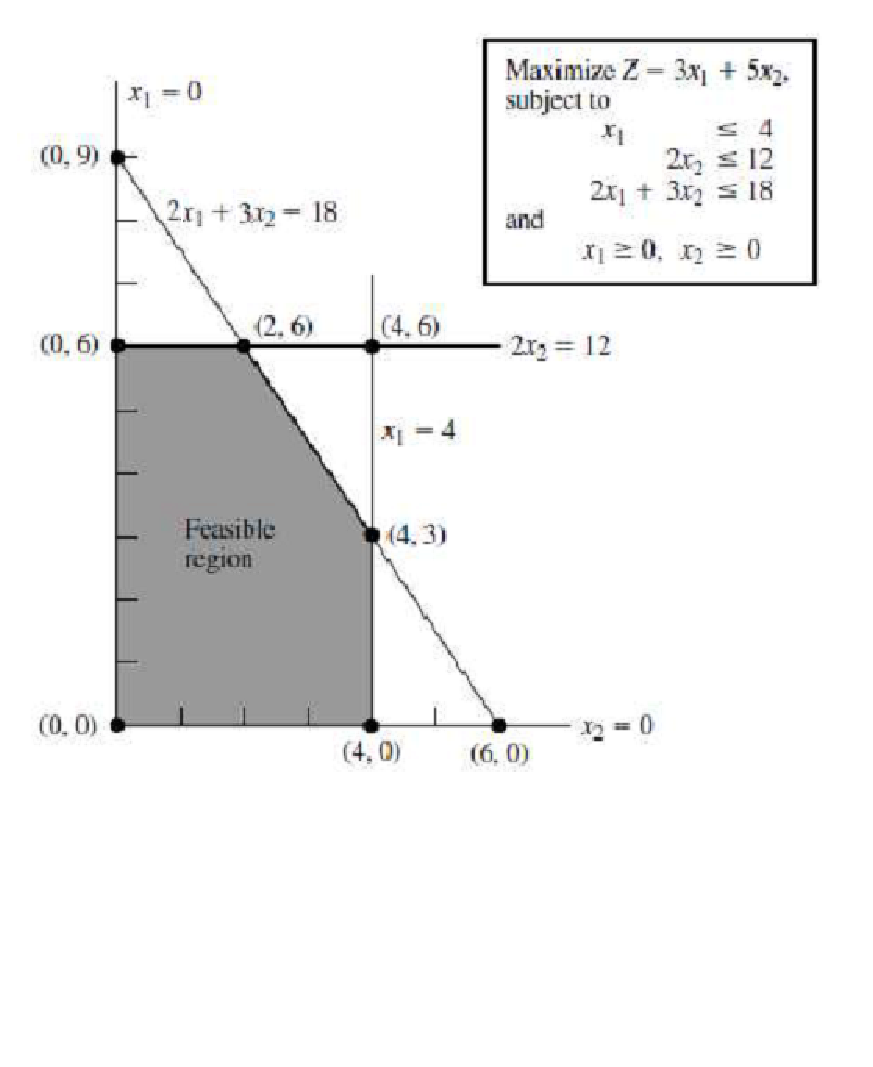
\includegraphics[scale=0.5]{graficos/Simplex_grafico_completo}
	\captionof{figure}{Um modelo de programação linear e a sua respectiva representação gráfica}
	\label{img:simplex_grafico_completo}
	\cite{Hillier}
\end{center}

Na figura \ref{img:simplex_grafico_completo} apresenta-se um exemplo de um problema de programação linear e sua representação geométrica. Nesse exemplo, de acordo com a representação geométrica do modelo, existem cinco possíveis soluções: x1=0 e  x2=0; x1=0 e  x2=6; x1=2 e  x2=6; x1=4 e  x2=3; x1=4 e x2=0. Como o objetivo é maximizar, concluímos que a melhor solução é x1=2 e  x2=6, em que z =36. No método Simplex a cada iteração, antes da solução ótima ser obtida, é encontrada uma dessas possíveis soluções que se localizam nos vértices do gráfico.

\section{Descrição do Método Simplex Revisado}
O método simplex revisado surgiu como uma solução para evitar cálculos desnecessários. Esse método foi projetado para problemas a serem solucionados computacionalmente.

No simplex revisado, são armazenados na memória volátil apenas os dados realmente necessários. Além disso, os cálculos são realizados apenas sobre a coluna que é utilizada na iteração, o que evita cálculos com matrizes que poderia acarretar uma imprecisão nos resultados.

Esse método mantém a característica do simplex, que é a troca entre a variável que entra na base e a que sai, além de também exigir certo esforço computacional. Porém sua grande vantagem é a economia de tempo e espaço, que garantida pelo modo como é desenvolvida a solução. 

Nesta seção descreve-se os passos do algoritmo simplex revisado. O problema considerado é de maximização. A distinção entre matrizes, vetores e escalares foi feita da seguinte forma: letra maiúscula e negrito para matriz (\textbf{MATRIZ}); letra minúscula e negrito para vetor (\textbf{vetor}); letra em itálico para escalar (\textit{escalar}).

Considere o seguinte problema de programação linear:

$\\
Maximizar\ \mathbf{cx} \\
Sujeito\ a \\
\mathbf{Ax} \leq \mathbf{b} \\
\mathbf{x} \geq0$

O vetor $\mathbf{c}$, de coeficientes na função objetivo, é dividido duas componentes: $\mathbf{c{_B}}$ e $\mathbf{c{_N}}$, coeficientes das variáveis básicas e não-básicas, respectivamente. Por analogia, o vetor $\mathbf{x}$, de incógnitas do problema, é subdividido em $\mathbf{x{_B}}$ e $\mathbf{x{_N}}$.  A matriz $\mathbf{A}$, de coeficientes das restrições, é dividida em duas submatrizes: $\mathbf{B}$ e $\mathbf{N}$, coeficientes das variáveis básicas e não-básicas, respectivamente. Os passos do algoritmo são os seguintes.\\

Passo 1: Calcular o valor das variáveis básicas: \ \ $\mathbf{x_{b}}\ =\ \mathbf{B^{-1}b}\geq0$

Passo 2: Calcular o vetor multiplicador: \ \ $\mathbf{\lambda} \ =\ \mathbf{c{_B}B^{-1}}$

Passo 3: Escolher a variável que entra na base. Para isso, calcula-se: $\mathbf{p}\ =\ \mathbf{c{_N}}-\mathbf{\lambda N}$

Se \ \ $\mathbf{p}\ =\ (\mathbf{c{_N}}-\mathbf{\lambda N})\leq 0$ \ \ PARAR.

A solução \ \ $\mathbf{x{_B}}$ \ \ já é a solução ótima. 

Caso contrário, escolher uma coluna de $\mathbf{N}$, coluna $\mathbf{a{_k}}$, tal que $\mathit{p{_k}}\ =\ \mathit{c{_nk}}-\mathbf{\lambda a{_k}}> 0$

Um critério frequente é escolher a coluna $\mathbf{a{_k}}$ que resulte no maior valor de $\mathit{p{_k}}$.

Então, assumindo $\mathit{e} = \mathit{k}$, $\mathit{k}$ representa o índice da coluna, $\mathbf{a{_k}}$ representa a coluna de $\mathbf{A}$ candidata a entrar na base. 

Passo 4: Determinar a variável que sai da base. Para isso, calcula-se: $\mathbf{y}=\mathbf{B^{-1}a{_k}}$

Se \ \ $\forall i\mathit{\frac{b{_i}}{y{_i}}}\leq 0$ \ \ PARAR.

A solução é não-limitada. Caso contrário, calcular:\ \ 
$\forall i\ \underset{\underset{y{_i}>0}{1\leq i\leq m}}{Min}\begin{Bmatrix}
\mathit{\frac{b{_i}}{y{_i}}}
\end{Bmatrix}$ e guardar o índice correspondente a $s = i$. A variável $(x{_b}){_s}$ sai da base.

Passo 5: Criar a matriz $\mathbf{E}$.
$\mathbf{E}=(\mathbf{e{_1}},\mathbf{e{_2}},...,\mathbf{e{_s-1}},\mathbf{\gamma} , \mathbf{e{_s+1}},...,\mathbf{e{_m}})$

Onde, cada coluna da matriz é um vetor unitário com exceção da coluna $\mathit{s}$, que corresponde ao vetor $\mathbf{\gamma}$, calculado da seguinte maneira: \\
$\mathbf{\gamma^{t}}=\left( \mathit{\frac{-\alpha {_{1,e}}}{\alpha {_{s,e}}}}\ \mathit{\frac{-\alpha {_{2,e}}}{\alpha {_{s,e}}}}\ ...\ \mathit{\frac{-\alpha {_{s-1,e}}}{\alpha {_{s,e}}}}\ \mathit{\frac{1}{\alpha {_{s,e}}}\ \frac{-\alpha {_{s+1,e}}}{\alpha {_{s,e}}}}\ ...\ \mathit{\frac{-\alpha {_{m,e}}}{\alpha {_{s,e}}}} \right )$

Onde $\mathit{\alpha{_ie}}$ são os elementos vetor do $\mathbf{y}$.

Passo 6: Calcular nova matriz $\mathbf{B^{-1}}$: $\mathbf{B^{-1}} = \mathbf{EB^{-1}}$

Passo 7: Atualizar os vetores $\mathbf{c{_B}}$ e $\mathbf{x{_B}}$.

\subsection{Método de Pontos Interiores}
Em 1984, Karmarkar revolucionou a área de programação linear com a publicação de um algoritmo de complexidade polinomial que apresentou bom desempenho quando aplicado a problemas práticos \cite{MaculanPI}. Essa publicação deu origem a um novo campo de pesquisa, chamado de método dos pontos interiores. 

O método de pontos interiores tem como principal característica realizar a busca por soluções no interior da região viável do problema, até encontrar a solução ótima \cite{Pinto}.
Em teoria, o método de pontos interiores é melhor que o método simplex, principalmente quando se leva em conta o critério de complexidade de pior caso. O método de pontos interiores possui complexidade polinomial, enquanto o método simplex possui complexidade exponencial No entanto, na prática ambos os métodos concorrem até hoje. Já que o sucesso do método depende da estrutura dos problemas, da esparsidade \footnote{Quando uma matriz possui uma grande proporção de elementos nulos diz-se que é uma matriz esparsa \cite{Munari}.} e da arquitetura dos computadores \cite{MaculanPI}.

\section{Aplicações Práticas}
Um problema de programação linear, como já dito anteriormente, busca a otimização na distribuição de recursos sujeitos a restrições. Por isso é considerada uma poderosa ferramenta de apoio a decisão \cite{FrossardMaxMin} e com utilização em diversas áreas, como: indústria, saúde, computação, produção, etc.
As empresas, por exemplo, devem estar constantemente atentas à competitividade e às restrições existentes com o objetivo de alcançar suas metas, para isso é necessário otimizar os recursos disponíveis \cite{FrossardMaxMin}. Daí a importância da utilização da programação linear empregada em seu exemplo mais geral: maximizar o lucro e minimizar custos.  Na definição de modelos desse tipo deve-se considerar o preço de venda e o custo de produção, além de restrições do tipo: quantidade de matéria- prima e mão-de-obra disponíveis, máquinas disponíveis para produção, entre outros \cite{FrossardMaxMin}.

\begin{citacao}
“Administrar com eficiência os recursos disponíveis na empresa, através do planejamento, controle e execução das atividades relacionadas á utilização destes, é fator fundamental na busca da otimização do resultado global da empresa. A programação linear juntamente com as técnicas de pesquisa operacional, permite identificar o resultado ótimo, considerando todas as restrições impostas no modelo adotado.” \cite[p.~31]{FrossardMaxMin}
\end{citacao}

Na computação, a programação linear é empregada, por exemplo, no processamento de imagens. Além disso é tema de estudos que buscam implementações eficientes de métodos de programação linear, em especial o método simplex, de forma distribuída ou integrada ao banco de dados.

\subsection{Aplicações em Processamento de Imagens}
O termo wavelet refere-se basicamente a um conjunto de funções com forma de pequenas ondas \cite{Ondaletas}. A decomposição wavelet é uma metodologia de decomposição de uma função ou sinal em um domínio de frequências e espaço, sendo possível investigar a ocorrência de fenômenos localizados no espaço e frequência simultaneamente \cite{Peixoto-wavelet}.
A decomposição wavelet em sua versão discreta é utilizada na compreensão de dados sendo útil no processamento de imagens quado é necessário realizar a extração de informações de um sinal e a análise de freqüências, principalmente quando ocorrem rápidas variações na frequência \cite{Leite-wavelet}

A decomposição wavelet tem sido abordada mediante diferentes métodos, como a Transformada de Fourier, por exemplo. Dentre eles estão presentes os métodos que tem como base a programação linear. Um dos primeiros trabalhos nesta área foi proposto por \citeonline{Chen} utilizando métodos de pontos interiores. Devido ao fato dos problemas lineares obtidos a partir da decomposição wavelet possuirem matrizes muito densas, os autores restringiram a pesquisa apenas ao caso de problemas com dicionários (conjunto de formas de ondas) com uma estrutura especial.  O método gera problemas lineares de grande porte, um problema de sinal de onda típico de comprimento 8192, por exemplo, se traduz em um problema linear de tamanho 8192 por 212.992.

No trabalho de \citeonline{YarmishWave} o autor resolve um conjunto de problemas de decomposição wavelet, utilizando tanto o método simplex revisado quanto o método simplex padrão. O autor mostra que embora o método simplex revisado seja superior no caso do problema mais geral (problema esparso), a resolução de problemas de decomposição wavelet resulta em um problema denso, onde o método simplex padrão tem melhor  desempenho.

Na figura \ref{img:ondaletas} são apresentados vários tipos de wavelets.

\begin{center}
	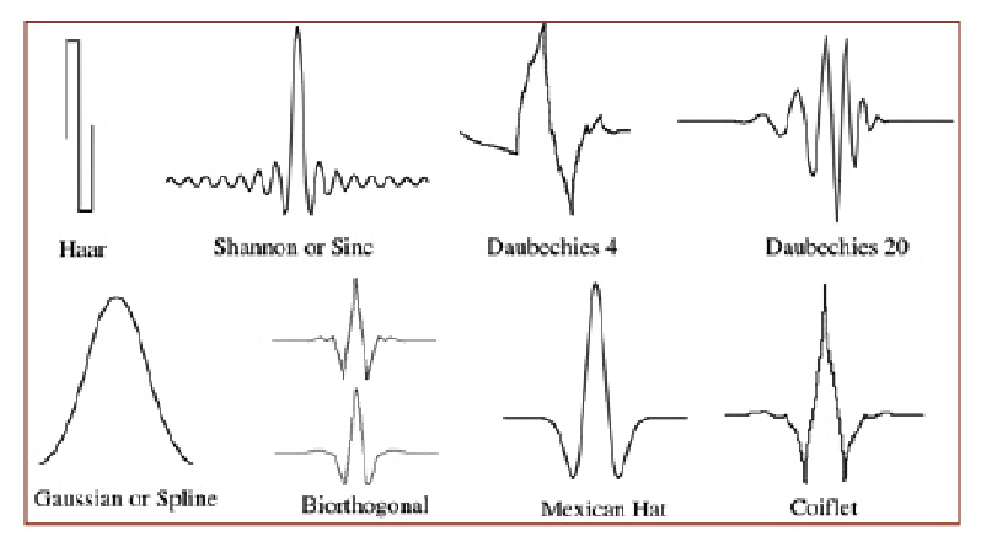
\includegraphics[scale=0.5]{graficos/ondaletas}
	\captionof{figure}{Exemplos de tipos de wavelets}
	\label{img:ondaletas}
 	\cite{FotoWave}
\end{center}

Em seu trabalho \citeonline{Komodakis} diz que problemas de análise de imagens podem ser formulados como problemas de rotulagem, onde a partir de uma imagem segmentada, são realizadas comparações entre pontos vizinhos a fim de rotular um grupo de pontos afins. Uma questão que vem incentivando pesquisas nessas áreas, é como resolver problemas desse tipo de forma eficiente e precisa. O autor propõe a utilização do esquema primal- dual da programação linear, e diz que essa utilização revelou excelentes resultados

\subsection{Aplicações em Programação Distribuída}
\citeonline{Slyke} e \citeonline{Yarmish-Distrubuido} demonstram a eficiência da utilização do método simplex padrão de forma distribuída. Esse método é mais utilizado e mais eficiente que o método revisado na resolução de problemas de grande porte, onde existe um maior volume de dados, fazendo mais sentido a utilização da programação distribuída.
De acordo com \citeonline{Slyke} e \citeonline{Yarmish-Distrubuido} a eficiência do método simplex revisado é afetada pela densidade do problema, ou seja, é uma método mais eficiente para problemas esparsos, os quais são mais comuns. Porém existem aplicações que exigem modelos mais densos, como em processamento de imagens. Nesse caso a implementação de uma algoritmo do método simplex padrão distribuído se mostra mais eficiente. Além disso, não existem algoritmos eficientes do método simplex revisado distribuído. Em conclusão o autor diz que a implementação apresentou bons resultados, especialmente para problemas grandes e densos.

Em \citeonline{Burger} é proposto um algoritmo simplex distribuído para problemas de programação linear degenerados e atribuições multi- agentes. Um problema de programação linear é dito degenerado se na solução uma das variáveis receber valor zero. O objetivo do trabalho é propor um algoritmo simplex para ser implementado em uma distribuição multi- agente, onde os a gentes devem concordar com uma solução ótima ou declarar o problema como inviável, caso não haja solução ótima.

Em seu trabalho \citeonline{Karypis} faz uma análise da performance de um algoritmo simplex paralelo em vários tipos de arquiteturas de rede, como por exemplo, rede hipercubo (Figura \ref{img:hipercubo}) e rede de estações de trabalho. Nesse tipo de implementação do método simplex, os dados da matriz são distribuídos entre os processadores que compõem a rede. Como resultado preliminar o autor obteve que na rede hipercubo a velocidade da resolução dos problemas cresceu a medida que mais processadores foram incorporados, inclusive para problemas de grande porte. Já na rede de estações de trabalho, para problemas pequenos a velocidade não teve um aumento proporcional ao aumento do número de processadores, enquanto que para problemas de maior porte a velocidade aumentou de forma proporcional ao número de processadores.

\begin{center}
	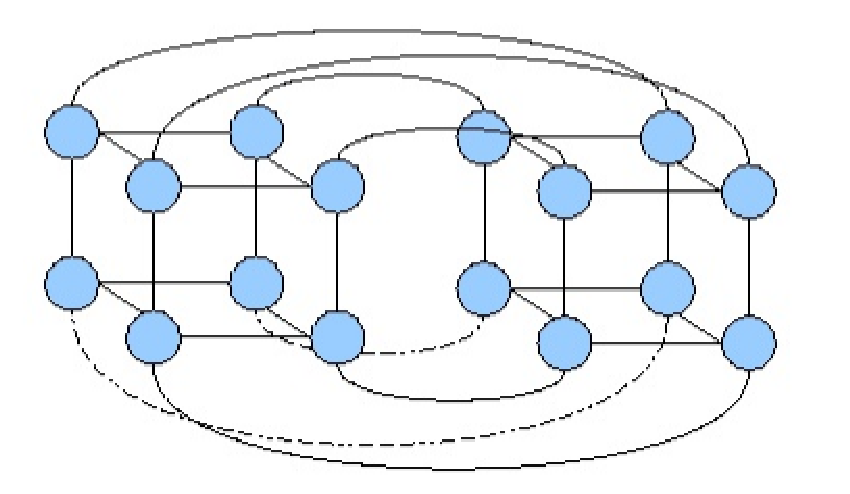
\includegraphics[scale=0.5]{graficos/hipercubo}
	\captionof{figure}{Na rede hipercubo com dimensão d, nesse caso d=4, cada nó está ligado a outros d nós, e o número de processadores é $2^{d}$}
	\label{img:hipercubo}
\end{center}

\subsection{Aplicações em Banco de Dados}
De acordo com \citeonline{Akira-database} dentre as inúmeras ferramentas de programação linear existentes, existe a carência de uma ferramenta que resolva problemas de programação linear de forma integrada a um banco de dados, utilizando procedimentos armazenados em sql pré-compiladas e armazenadas no banco de dados juntamente com os dados. Essa características em uma ferramenta se torna importante, principalmente, em problemas de grande porte, suprimindo o tráfego de dados já que toda a lógica é executada internamente no banco de dados, e apenas o resultado final é enviado para o usuário. Na implementação apresentada por \citeonline{Akira-database} os dados do modelo a ser resolvido são armazenados como modelos relacionais, ou seja, em matrizes bi-dimensionais. Apesar das vantagens desse tipo de implementação, o autor chegou a conclusão que o tempo de execução ainda deve ser melhorado.

\subsection{Aplicação em Saúde}
A programação linear também se aplica na área da saúde, em \citeonline{Alterovitz-saude} é feita uma proposta de utilização da programação linear no tratamento do câncer. 
Em um determinado tipo de tratamento são inseridos cateteres na área afetada para introduzir o medicamento necessário, porém o medicamento acaba afetado células saudáveis além das cancerígenas. Como os problemas de programação linear podem ser resolvidos como problemas determinísticos e com solução exata, \citeonline{Alterovitz-saude} propõe que a formulação de um problema de otimização para determinar o tempo de permanência dos cateteres, minimizando os desvios na quantidade da dose necessitada pelo paciente. Nos testes realizados, os resultados obtidos não mostraram uma vantagem significativa em relação ao método atualmente utilizado.

\subsection{Aplicação no reconhecimento de expressões faciais}

Em seus trabalhos, \citeonline{Feng} e \citeonline{Guo} apresentaram uma abordagem de reconhecimento de expresssões faciais utilizando a programação linear. Em ambos a programação linear foi utilizada na fase de classificação da expressão. Em \citeonline{Guo} a programação lienar foi utlizada ainda na fase de extração de carcaterísticas, para determinar a quantidade de caracteríticas a serem selecionadas e os principais pontos da face. Enquanto no trabalho de \cite{Feng} é utilizado o filtro de Gabor na etapa de extração de carcaterísticas. O Filtro de Gabor tem a capacidade de realçar bordas e saliências na imagem. Após a aplicação do filtro na imagem, são realçadas as características salientes presentes no rosto (cantos dos olhos, cantos da boca, narinas, entre outros) \cite{Gabor}. Em ambos os trabalhos foram obtidos ótimos resultados e superiores a outros métodos com os quais foram comparados. 

A programação linear é utlizada na etapa após o tratamento da imagem. Primeiramente as expressões são combinadas em pares. No trabalho de \cite{Feng}, por exemplo, busca-se o reconhecimento de sete expressões: raiva, desgosto, medo, felicidade, tristeza, surpresa e neutro. Essas expressões são combinada em pares do tipo: raiva-desgosto, raiva-medo, etc. Formando um total de 21 pares. Após isso o modelo de programação linear, apresentado mais adiante, é utilizado para gerar os calssificares, o modelo deve ser rodado 21 vezes, uma para cada par de expressões. Essa etapa é também chamada de treinamento, pois a partir do classificadores gerados as expressões das imagens a serem analisadas serão determinadas. Essa abordagem também substitui a utilização de redes neurais para o treinamento, uma vantagem é que o modelo necessita ser rodado uma única vez para cada par, enquanto em uma abordagem utilizando redes neurais este processo se trona iterativo.

Na última etapa de determinação da exepressão é utilizda uma estrtura de árvore binária de torneio.

\subsection{Aplicações na Engenharia de Produção}
Dentre as aplicações mais conhecidas da programação linear, encontram-se os problemas de planejamento de produção e controle de estoque e os problemas de mistura. Os problemas do primeiro tipo possuem inúmeras aplicações, desde a alocação de máquinas para atender determinada demanda, até a utilização do estoque para atender a uma mudança imprevisível na demanda e necessidades de contratação de demissão para enfrentar mudanças nas necessidades de mão de obra. Já os problemas de mistura tratam, basicamente, da mistura de diferentes matérias para a produção de produtos, que devem obedecer a algumas especificações e, ao mesmo tempo, minimizar o custo ou maximizar o lucro.  \cite{Taha}.
Um exemplo mais prático seria a produção de rações animais onde o objetivo é minimizar o custo de produção da ração composta por dois ingredientes. Estando restrito a quantidade total que deve ser produzida, além das quantidades de nutrientes necessários.

 $\\Minimize\ z=0,9x_{1}+0,5x_{2}\\
Sujeito\ a\\$
\begin{eqnarray*}
        x_{1}+x_{2}\geq 90 \ (a)\\
        0,09x_{1}+0,05x_{2}\geq 0,07(x_{1}+x_{2}) \ (b)\\
        0,02x_{1}+0,06x_{2}\geq 0,03(x_{1}+x_{2}) \ (c)\\
         x_{1}\geq 0 \ (d)\\
	 x_{2}\geq 0 \ (e)
\end{eqnarray*}

Onde, 
\begin{itemize}
\item \textbf {x1} representa a quantidade do ingrediente 1 que a ração deve conter
\item \textbf {x2} representa a quantidade do ingrediente 2 que a ração deve conter
\item \textbf {Z} representa o custo total da produção dessa ração, sendo que o custo (por grama) do ingrediente 1 é de R\$ 0,9 e o custo (por grama) do ingrediente 2 é de R\$ 0,5
\end{itemize}

E as restrições representam as restrições das quantidades de nutrientes que a ração deve conter e a quantidade total,
\begin{itemize}
\item \textbf {(a)} representa a quantidade total de ração que deve ser produzida (em quilos)
\item \textbf {(b)} representa que a ração deve conter 7\% de um determinado nutriente, e 9\% de cada grama do ingrediente 1 e 5\% de cada grama do ingrediente 2 é composto por esse nutriente. 
\item \textbf {(c)} representa que a ração deve conter 3\% de um determinado nutriente, e 2\% de cada grama do ingrediente 1 e 6\% de cada grama do ingrediente 2 é composto por esse nutriente.
\item \textbf {(d)} representa que a ração deve conter o ingrediente 1
\item \textbf {(e)} representa que a ração deve conter o ingrediente 1
\end{itemize}

A programação linear além de estar presente, é fundamental em diversas áreas, tornando-se uma ferramenta de apoio a decisão e contribuindo para o sucesso de projetos nas áreas em que se aplica.

\section{Métodos de Classificação}
Em problemas de calssificação, dado um conjunto de dados de treinamento onde cada subconjunto pertence a uma entre n classes, o objetivo é que dada uma instância o método de classificação retorne a qual das n classes essa instância pertence. A seguir são apresentados alguns dos métodos mais citados na literatura. 

\subsection{Support Vector Machines}
Support Vector Machines ou Máquinas de vetores de suporte (SVM) têm a capacidade de gerar classificadores na etapa de treinamento e de classificar os dados na etapa de teste de acordo com o classificadores gerados. Considerando um problema de classificação com duas classes, uma SVM irá determinar um plano que separe os pontos dessas duas classe, de forma que a distância entre o hiperplano e os pontos seja a máxima possível. Os pontos de cada classe utlizados como referência são denominados vetores de suporte.
No caso de conjuntos linearmente inseparáveis, é utilizada um função denominada Kernel. Essa função é responsável por elevar a dimensão espacial a fim de que os pontos se tornem linearmente separáveis.Portanto a obtenção de um classificador por meio do uso de SVM é necessária a escolha de uma função kernel e os parâmetros dessa função. Essa esolha influencia diretamente no desempenho do classificador\cite{Gunn98SVM}\cite{Reffson02SVM}.

FIGURA!!!!!!!!!!

No caso em que é o núemro de classes é maior que dois, duas abordagens podem ser utilizadas com as SVM \cite{Lorena03SVM}:
\begin{itemize}
\item{Um contra todos: }Nessa abordagem, para K padrões são geradas K SVM. Na criação das SVM, é gerado um hiperplano que separa 1 classe das k-1 classes. Na determinação do padrão de uma instância x, o padrão é aquele que, entre as k SVM obteve mais mais valores de x do lado do hiperplano onde se encontrava o padrão k.  
\item{Todos contra um: }Nessa abordagem os padrões são agrupados em pares e uma SVM é gerada para cada par. Um esquema de votação deve ser utilizado para determinar o padrão de uma instância, que deve ser analisada a partir de cada SVM e cada SVM retorna uma classe possível. A classe que obtiver mais pontos da instância é a classe atribuída.
\end{itemize}

\subsection{Naive Bayes}
Na metodologia Naive Bayes as carcterísticas do dado a ser classificado são analisadas de forma independente. O vetor de característcas é formado pela número de vezes que cada característica ocorre no dado caracterizado. A probabilidade de uma instância pertencer a um determinado padrão é dada por uma probabilidade inicial, baseada na quantidade total de dados, e pelas probabilidades das ocorrências das características. Essa abordagem é mais comunmente utlizada na área de mineração de dados, onde dada uma palavra busca-se o melhor texto baseado nas probabilidades de aparecimento da palavra no textos utilizados no treinamento \cite{McCallum98Bayes}\cite{Langley92Bayes}.

\subsection{k- nearest neighbor}
Nesse método a classificação é feita pela similaridade da instância a ser classificada com um dado utlizado no treinamento, a classe do dado utilizado no treinamento é então atribuída a instância com padrão inicalmente desconhecido. As estapas desse métodos consistem em utilizar um parâmetro para medir a semelhança ou a distância do dado a ser classificado em relação a cada um dos dados utlizados no treinamento. Os mais similares ou mais próximos são selecionados e entre esses um é escolhido e o seu padrão é atribuído ao dado incialmente desconhecido. Apesar de ser considerado um método simples, sua dificuldade está em definir os parâmetros que definiram a semelhança entre os dados\cite{Chagas09KNN}.
COLOCAR FIGURA!!!!!

\section{Métodos de validação do modelo}
Um modelo de classificação pode ser verificado em relação a sua acurácia apartir de um conjunto de dados ou a sua performance em relação a outros métodos classificadores podem ser verificados. Algumas técnicas utilizadas com esse intuito serão apresentadas a seguir. No presente trabalho a técnica Cross Validation é utilizada com o objetivo de verificar a acurácia, nesse caso, da metodologia utlizada na classificação de padrões \cite{Kohavi95Cross} \cite{Baldisserotto05Validacao}.
A seguir são apresentadas as três técnicas mais comumentes encontradas na bibliografia com suas ventagens e desvantagens:

\subsection{Handout}
Esse é um método simples, onde os dados são divididos em 2 grupos mutuamente exclusivos, sendo um grupo utilizado para treino e o outro para teste. Em geral 2/3 dos dados são utilizados no treinamento e 1/3 na etapa de testes. É mais indicado quando uma grande quantidade de dados está disponível, de forma que os dois grupos possam conter dados suficientes de todos os padrões, nesse caso, suficientes para que o resultado final não seja comprometido pela falta de dados no grupo da etapa de treino e nem no grupo de testes. Apesar de ser um método de fácil implementação, a divisão entre conjunto de treinamento e teste deve ser bem estudada de forma que todos os padrões estejam bem representados nos dois grupos, por isso é um método recomendável quando o conjunto de dados possui um grande número de representações de cada padrão \cite{Kohavi95Cross} \cite{Baldisserotto05Validacao}.

\subsection {Cross Validation}
Nesse método, o conjunto de dados também é dividido em cojunto de treinamento e de teste, porém esses dois grupos variam a cada rodada de teste. O tipo de cross validation mais comumente utilizado é o k-fold cross validation, onde os dados são divididos em k conjuntos mutuamente exclusivos e as etapas de treinamento e teste são realizdas K vezes, de forma que a cada rodada um conjunto diferente é utilizado como teste e os outros k-1 conjuntos são utilizados para treinamento. Esse método é recomendável quando o conjunto de dados não é tão grande, pois não existe uma  preocupação de quais dados separar para teste e quais separar para validação, já que a ao final da execução do método todos o dados terão participado dos conjuntos de validação e teste \cite{Kohavi95Cross} \cite{Baldisserotto05Validacao}.

\subsection{Leave-one-out}
Nessa técnica, do conjunto com o número total de dados N, são realizadas N rodadas de treinamento e teste, sendo que a cada rodada N-1 dados são utlizados para teste e o dados restante é utlizado para treinamento. Pelas suas características, esse é um método recomendável para conjuntos de dados pequenos já que a quantidade de rodadas de treinamento e teste é igual a quantidade de dados o que o torna um método com alto custo computacional \cite{Kohavi95Cross} \cite{Baldisserotto05Validacao}.

\section{Trabalhos Relacionados}
Em seu trabalho \citeonline{Reffson02SVM} busca o classificação de impressões digitais em 5 classe. Esse tipo de classificação tem o próposito de gerenciar grandes bancos de dados de impressões digitais e acelerar o processo de identificação. Foi utilizado um banco contendo 4000 imagens igualmente distribuídas entre as cinco classes. O autor dividiu o banco em dois grupos, utilizando um para treinamento e outro para teste. Após a extração das características das imagens, Máquinas de Vetores de Suporte foram utlizadas na classificação. Na abordagem todos contra um foi obtida uma média de precisão de 91,18\%, já na abordagem um contra todos a precisão na classificação das impressões foi de 90,43\%.

\citeonline{Chagas09KNN} apresentou uma técnica para a classificação de textos, uma atividade importante em aplicações como bibliotecas digitais e em outras que em geral buscam a organização de documentos disponíveis no formato digital. O autor propôs variações no método K near neighbor a fim de  aprimorar a escolha dos textos utilizados no treinamento mais próximos ao texto que precisa ser classificado. Nos testes feitos com três coleções de textos, as médias de acertos na classificação obtidas foram acima de 90\% em duas coleções, e próxima a 70\% na terceira.

Em \citeonline{Feng} foi realizado um estudo de reconhecimento de expressões faciais, utilizando a base de dados JAFFE \cite{Jaffe}, em uma etapa de pre processamento as coordenadas do olhos foram marcadas manualmente e utilizando uam máscara elíptica as imagens foram reduzidas a região da face. Na extraçãod e características foi utilizado o método local binary patterns. O modelo de programação linear proposto em \cite{Bennett92robustlinear} é utlizado para gerar os classificadores e na classificação de imagens com expressão desconhecida foi utilizada uma árvore de torneio. Para validação os dados foram divididos em 10 conjuntos, o ciclo de treinamento e teste foi repetido 10 vezes, sendo que em cada ciclo um conjunto foi usado como teste e os outros nove para validação. Foram realizados 20 desses ciclos e uma média da taxa de acertos foi calculada, obtendo uma taxa de 93.8\%. Os autores concluíram que o método obteve uma performance excelente comparado a outros estudos de receonhecimento de expressão facial que utilizaram a mesma base de dados.
